\section{Appendix}
\begin{figure}[tbh]
    \centering
    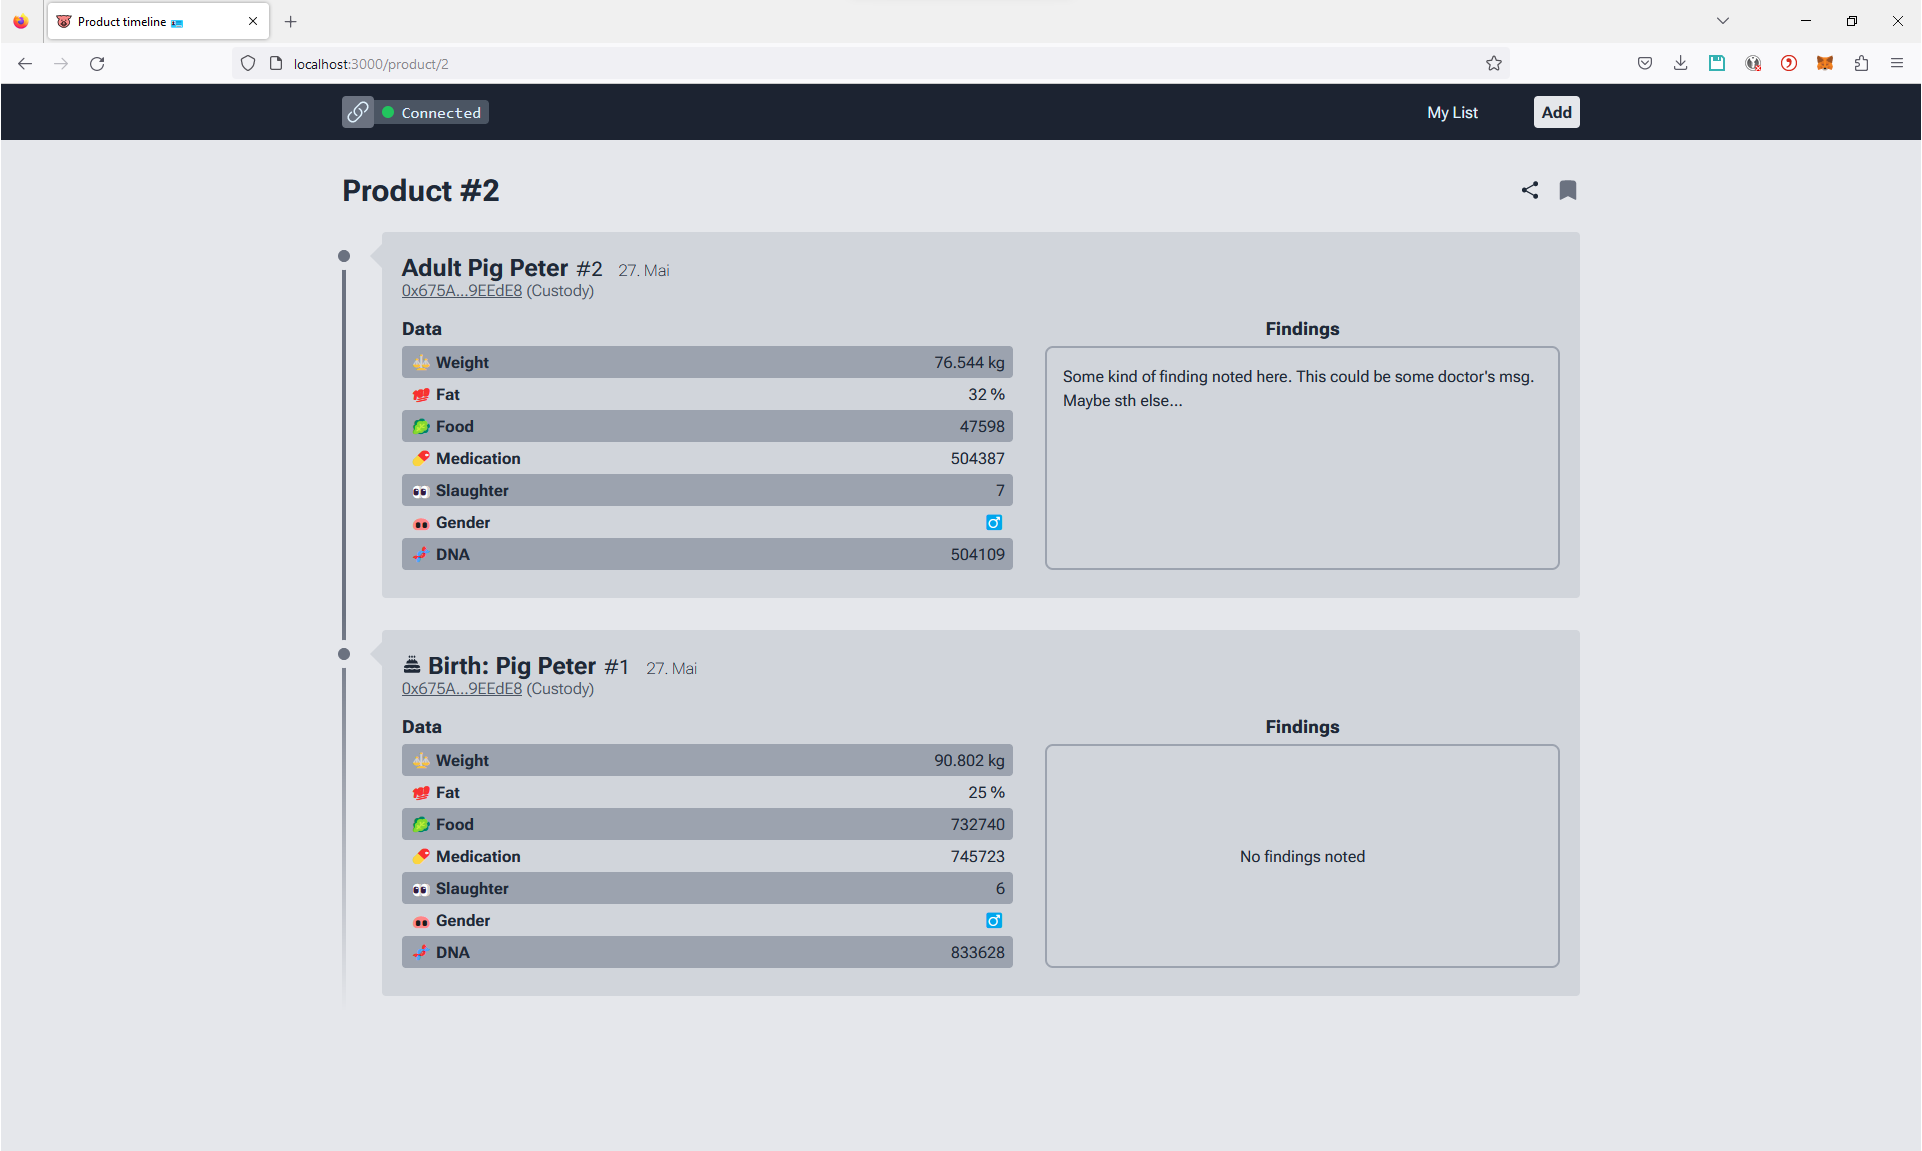
\includegraphics[width=0.82\textwidth]{images/timeline.png}
    \caption{Timeline of a product's chain}
    \label{fig:timeline_pig}
\end{figure}

\begin{figure}[tbh]
    \centering
    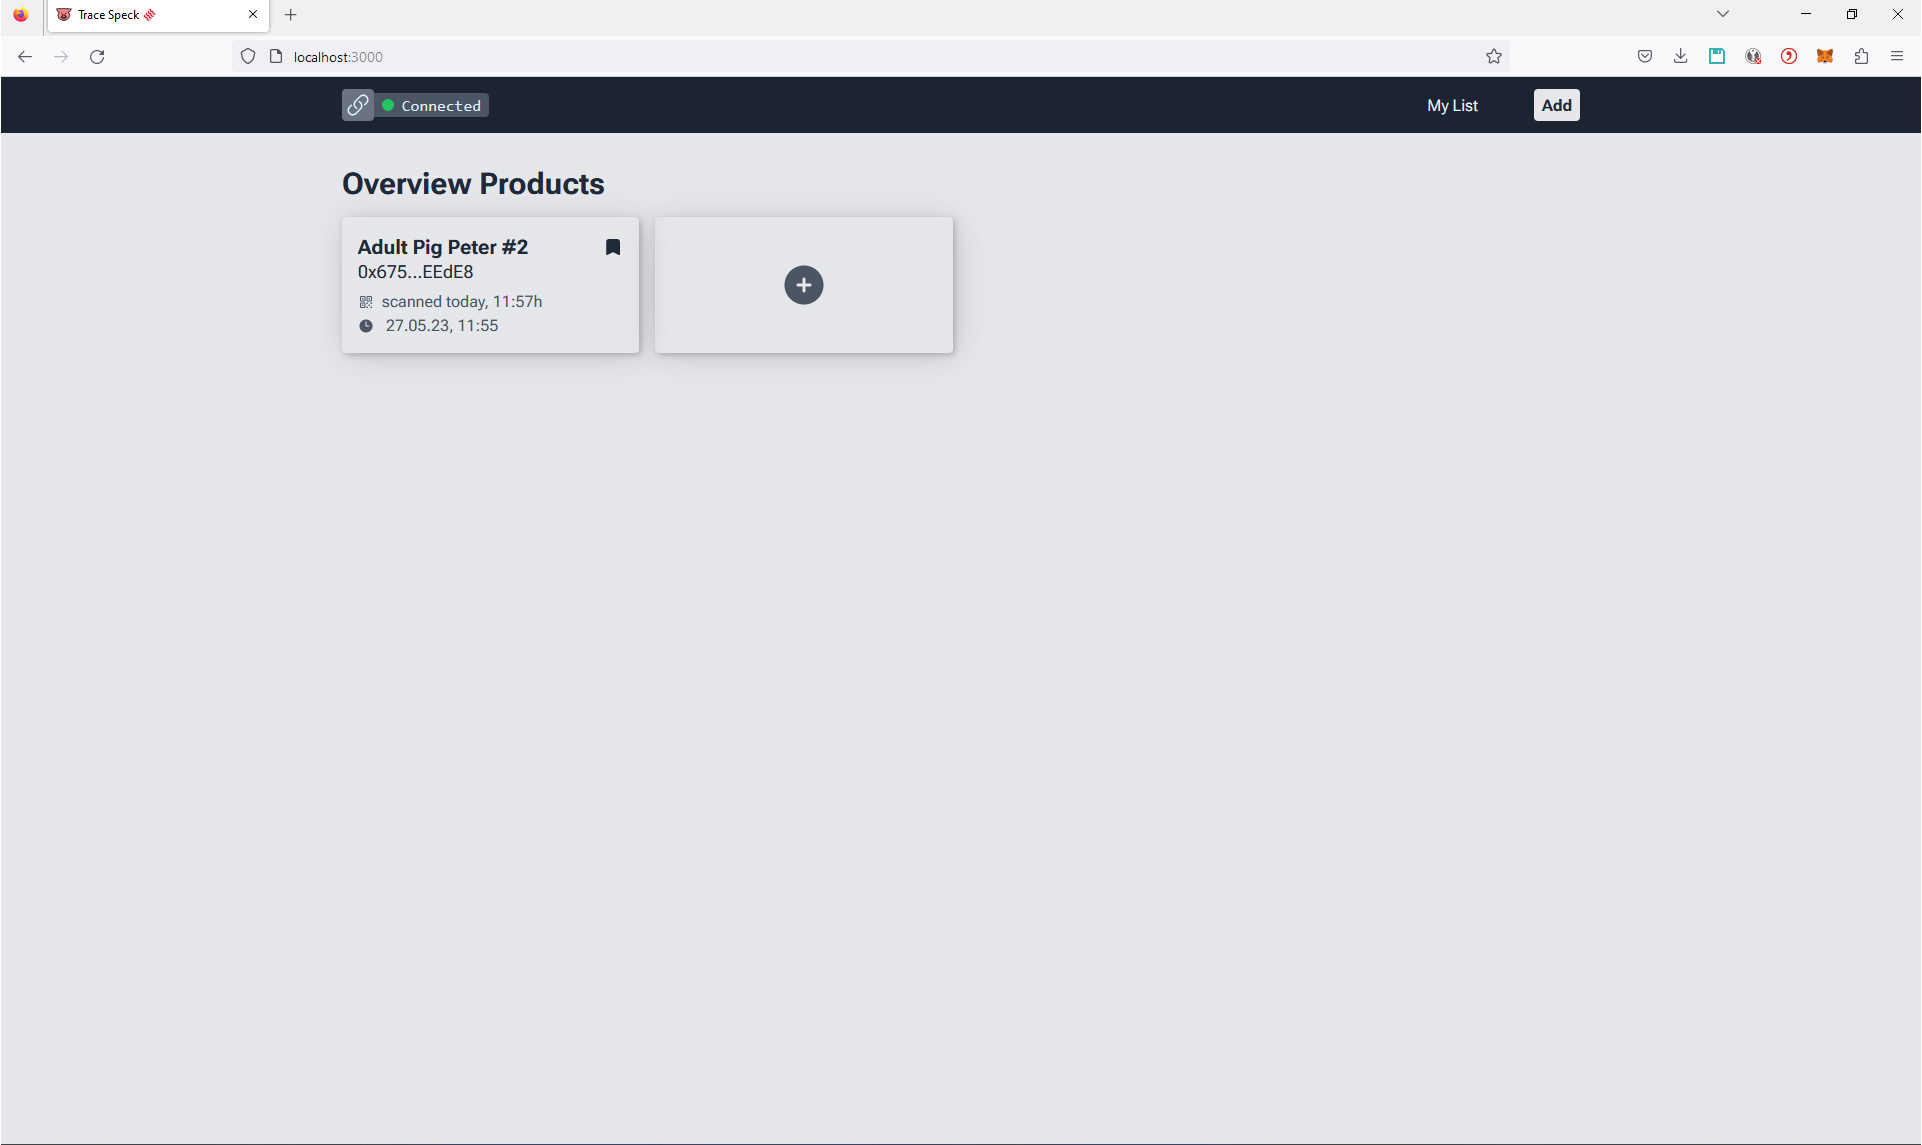
\includegraphics[width=0.82\textwidth]{images/list_pigs.png}
    \caption{Collection of pigs that added to watchlist by consumer}
    \label{fig:list_of_pigs}
\end{figure}


\begin{figure}[tbh]
    \centering
    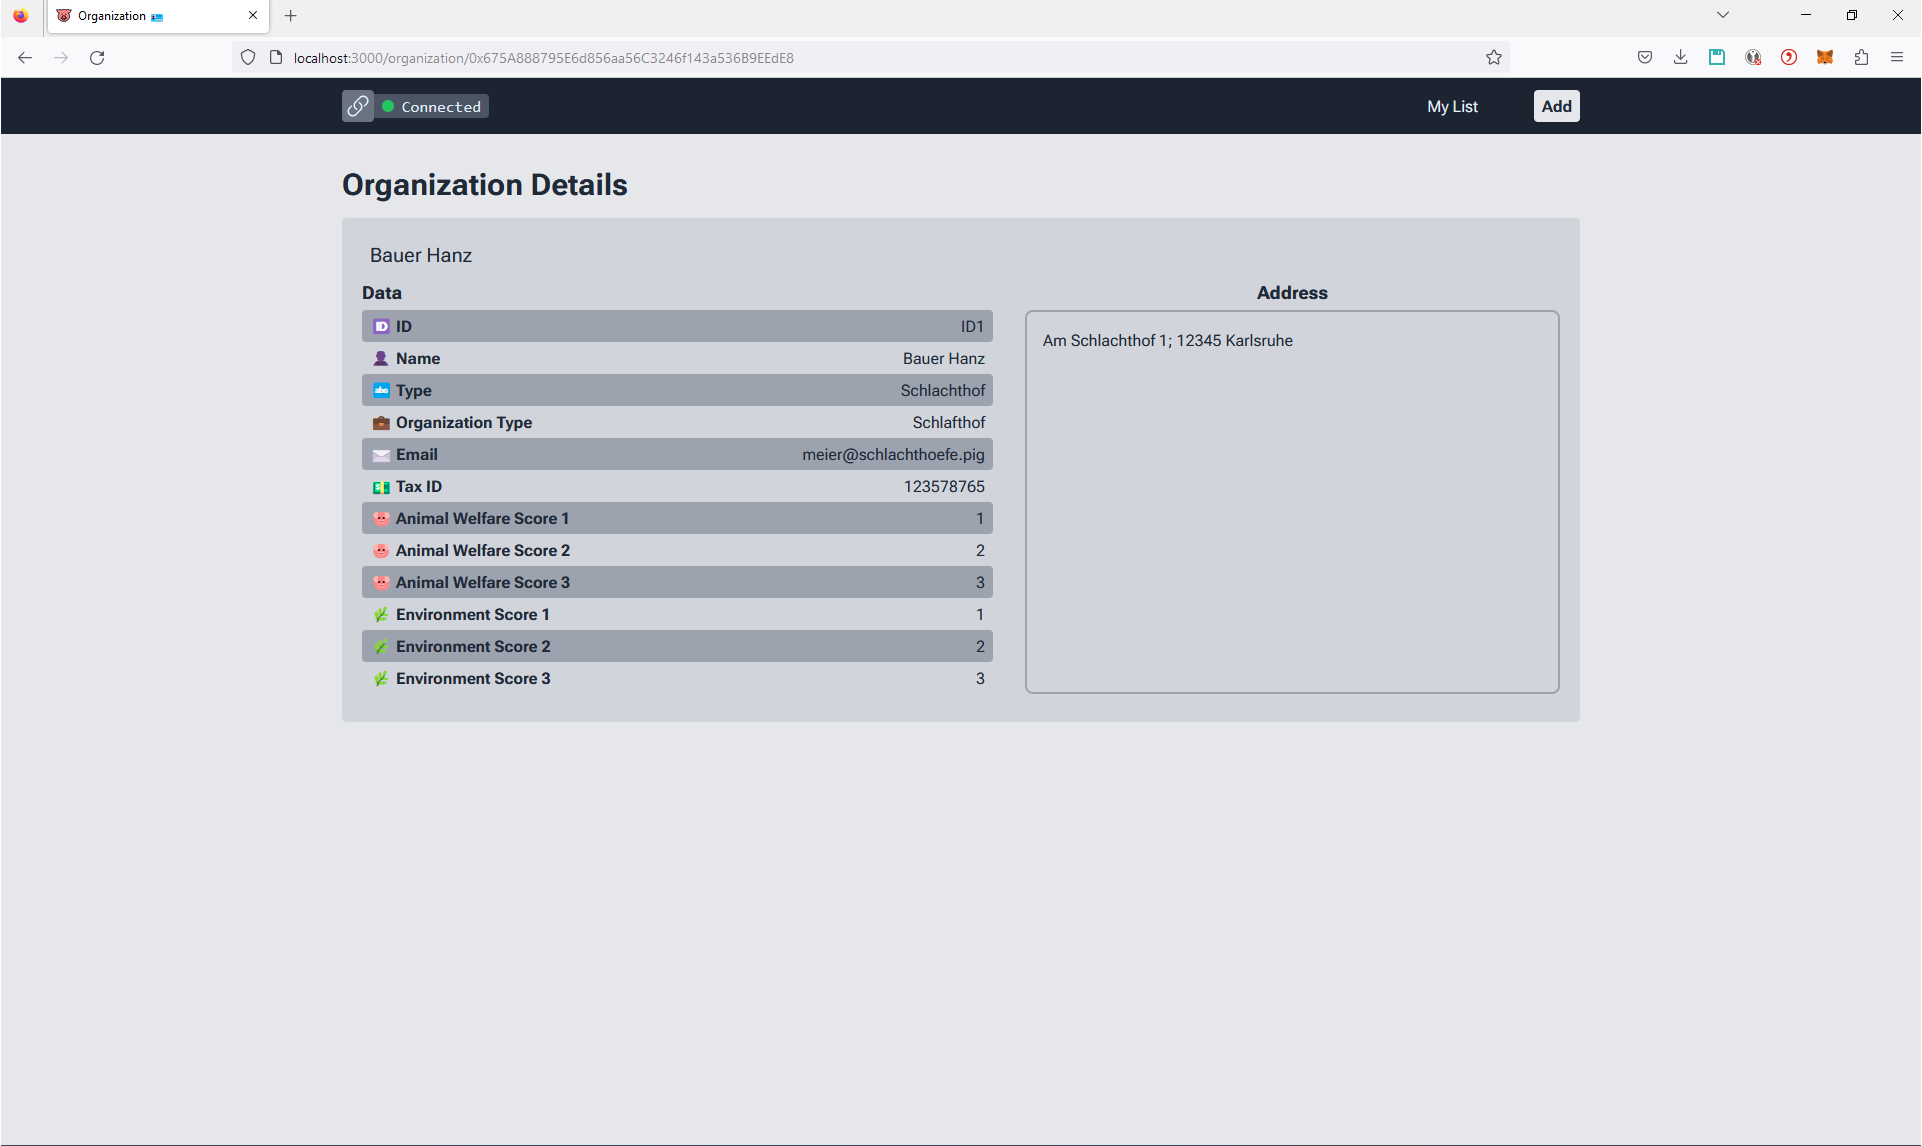
\includegraphics[width=0.82\textwidth]{images/oragnization.png}
    \caption{Registered organization displayed to consumer}
    \label{fig:organization}
\end{figure}

\begin{figure}[bth]
    \centering
    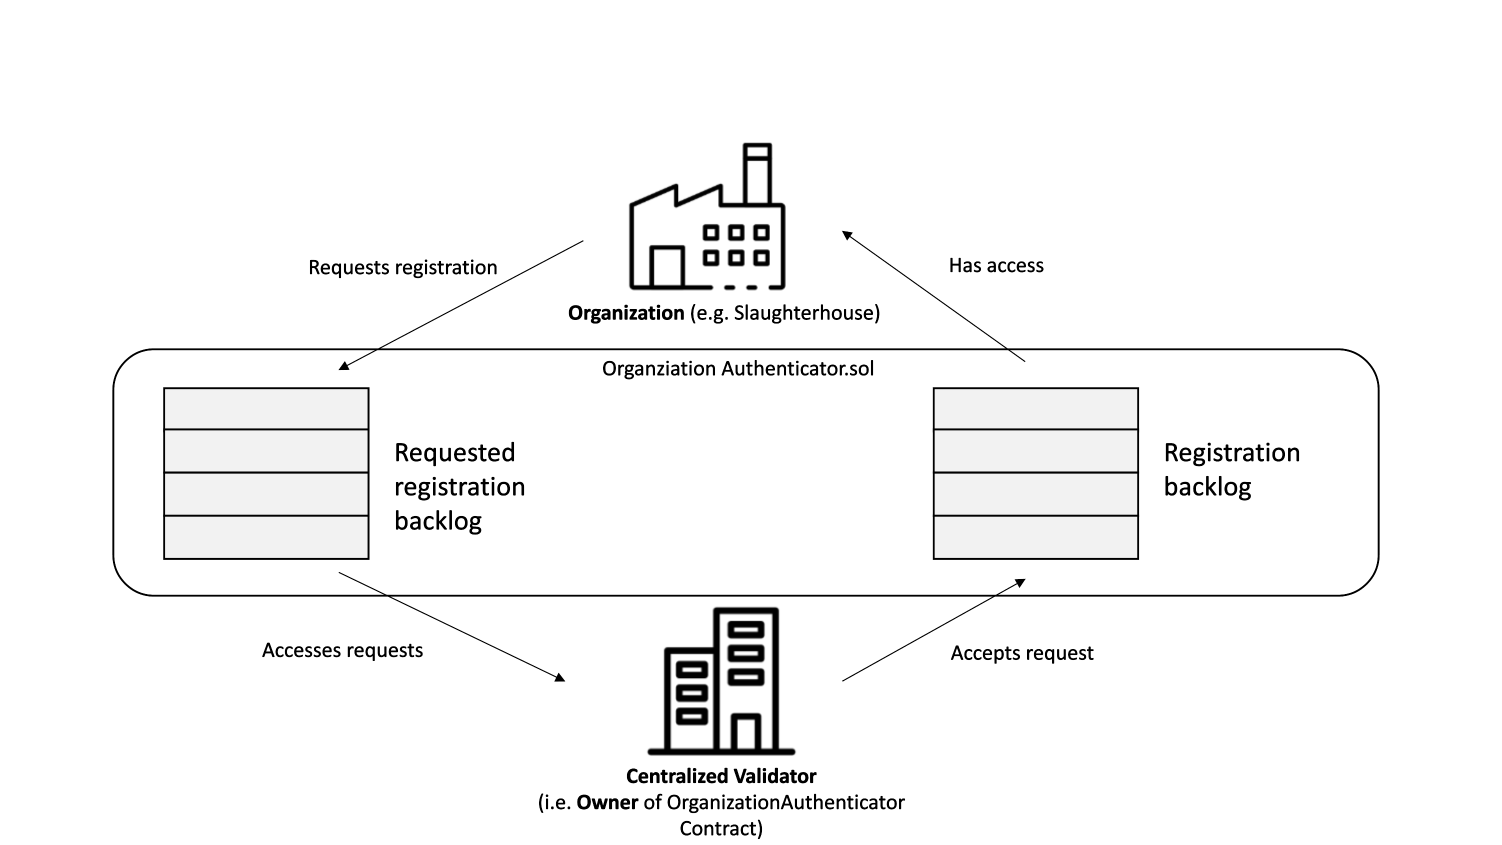
\includegraphics[width=1\textwidth]{images/registration_process.png}
    \caption{Registration process of \textit{OrganizationAuthenticator.sol}}
    \label{fig:registration_process}
\end{figure}

\newpage
\subsection{OrganizationAutheticator.sol}\label{se:organization_authenticator.sol}


\textbf{Imports}

\begin{itemize}
    \item "@openzeppelin/contracts/token/ERC721/ERC721.sol"
    \item "@openzeppelin/contracts/utils/Counters.sol"
    \item  "@openzeppelin/contracts/access/Ownable.sol"
\end{itemize}


\textbf{State Variables}


\begin{table}[H]
\resizebox{\columnwidth}{!}{%
\begin{tabular}{ll}
\textbf{Name}              & \textbf{Description}                                                                   \\
\texttt{\textunderscore orgIds}                    & A counter to track the next open token ID     \\
\texttt{\textunderscore organizationAuthenticator}             & A counter to track the number of registration requests.                                \\
\texttt{\textunderscore registeredAmount}           & A counter to track the number of registered organizations.                             \\
\texttt{\textunderscore registered}                 & A mapping to store the registration status of organizations based on their ID.         \\
\texttt{\textunderscore organizationData}           & A mapping to store organization data based on their ID.                                \\
\texttt{\textunderscore registrationRequested}      & A mapping to track the registration request status of organizations based on their ID. \\
\texttt{\textunderscore addressToId}                & A mapping to associate an organization's Ethereum address with its ID.                 \\
\texttt{\textunderscore registrationRequestedArray} & An array to store the IDs of organizations that have requested registration.          
\end{tabular}%
}
\end{table}

\textbf{Events}


\begin{itemize}
    \item \texttt{\textunderscore Authenticate(string \textunderscore msg)}: Event emitted when an authentication is performed.
    \item \texttt{\textunderscore RegistrationRequested(address indexed requestAddress)}: Event emitted when a registration request is made.
\end{itemize}



\textbf{Structs}

\texttt{Organization}: A struct to hold organization data
\begin{table}[H]
\begin{tabular}{ll}
\textbf{Attribute}     & \textbf{Datatype} \\
\texttt{id}                     & string            \\
\texttt{name}                   & string            \\
\texttt{type\textunderscore}                  & string            \\
\texttt{organization\textunderscore type}      & string            \\
\texttt{email}                  & string            \\
\texttt{institution\textunderscore type}       & string            \\
\texttt{address\textunderscore}              & string            \\
\texttt{tax\textunderscore id}                 & uint256           \\
\texttt{animal\textunderscore welfare\textunderscore score\textunderscore 1} & uint256           \\
\texttt{animal\textunderscore welfare\textunderscore score\textunderscore 2} & uint256           \\
\texttt{animal\textunderscore welfare\textunderscore score\textunderscore 3} & uint256           \\
\texttt{environment\textunderscore score\textunderscore 1}    & uint256           \\
\texttt{environment\textunderscore score\textunderscore 2}    & uint256           \\
\texttt{environment\textunderscore score\textunderscore 3}    & uint256           \\
\texttt{creation\textunderscore right}        & bool             
\end{tabular}
\end{table}




\textbf{Modifiers}
\begin{itemize}
      \item \texttt{\textunderscore onlyOwner} \textit{(from ERC721)}: Modifier that restricts access to the contract owner.
\end{itemize}

\textbf{Methods}
\begin{table}[H]
\resizebox{\columnwidth}{!}{%
\begin{tabular}{lll}
\textbf{Name} &                   & \textbf{Description}                                                                                           \\ \hline
\texttt{authenticateById} & \textbf{@dev}     & Check if the organization with the given ID is registered.                                       \\
                          & \textbf{@params}  & \texttt{\_orgId}: ID of the organization to check authentication status.                                         \\
                          & \textbf{@returns} & A boolean indicating if the organization is registered or not.                                       \\
                          &                   &                                                                                                                \\ \hline
\texttt{authenticate} & \textbf{@dev}     & Check if the organization with the given address is registered.                                                    \\
                          & \textbf{@params}  & \texttt{\_address}: Address of the organization to check authentication status. \\
                          & \textbf{@returns} & A boolean indicating if the organization is registered or not.                                                 \\
                          &                   &                                                                                                                \\ \hline
\texttt{requestRegistration} & \textbf{@dev}              & Request registration for a new organization.                                                                   \\
                          & \textbf{@params}           & \texttt{\_data}: Struct containing organization data to register                                                           \\
                          &                   &                                                                                                                \\ \hline
\texttt{register} & \textbf{@dev}              & Register an organization.                                                                                      \\
                          & \textbf{@params}           & \texttt{\_orgId}: ID of the organization to register                                                                     \\
                          &                   &                                                                                                                \\ \hline
\texttt{getRequestedRegistrations} & \textbf{@dev}              & Get a list of organization requests.                                                                           \\
                          & \textbf{@returns}           & An array of organizations                                                                                          \\
                          &                   &                                                                                                                \\ \hline
\texttt{getMyData} &      \textbf{@dev}        & Get the organization data from \textit{msg.sender}                                                           \\
                          & \textbf{@returns}           & Organization data of the \texttt{msg.sender}                                                                     \\
                          &                   &                                                                                                                \\ \hline
\texttt{amIRegistered} &        \textbf{@dev}      & Check if the \textit{msg.sender} is registered                                                             \\
                          & \textbf{@returns}           & A boolean indicating if the \texttt{msg.sender} is registered or not                                                                      \\
                          &                   &                                                                                                                \\ \hline
\texttt{getOrganizationDataByAddress} &      \textbf{@dev}        & Get the organization data of a given address                                                                 \\
                          & \textbf{@params}           & \texttt{\_address}: Address of the organization to retrieve data for                                                           \\
                          & \textbf{@returns}           & Organization data of the given address                                                                 \\
                          &                   &                                                                                                                \\ \hline
\texttt{totalRequestedOrganizationAmount} &      \textbf{@dev}        & Get the total number of organization registration requests                                                                           \\
                          & \textbf{@returns}           & The total number of organization registration requests                                                                      \\
                          &                   &                                                                                                                \\ \hline
\texttt{totalRegisteredOrganizationAmount} &      \textbf{@dev}        & Get the total number of registered organizations                                                                 \\
                          & \textbf{@returns}           & The total number of registered organizations                                                                      \\
                          &                   &                                                                                                                \\ \hline
\end{tabular}%
}
\end{table}

\newpage
\subsection{Speck.sol}\label{se:speck.sol}
\textbf{Imports}

\begin{itemize}
    \item "@openzeppelin/contracts/token/ERC721/ERC721.sol"
    \item "@openzeppelin/contracts/utils/Counters.sol"
    \item  "@openzeppelin/contracts/access/Ownable.sol"
\end{itemize}


\textbf{State Variables}


\begin{table}[H]
\resizebox{\columnwidth}{!}{%
\begin{tabular}{ll}
\textbf{Name}              & \textbf{Description}                                                                   \\
\texttt{\textunderscore tokenIds}                    & A counter to track the next open token ID.      \\
\texttt{\textunderscore organizationAuthenticator}             & Instance of the OrganizationAuthenticator contract.                                \\
\texttt{\textunderscore products}           & A mapping for storing product data.                           \\
\texttt{\textunderscore tokenOwner}                 & A mapping for storing the owner of a product.        \\       
\end{tabular}%
}
\end{table}

\textbf{Events}
\begin{itemize}
    \item \texttt{\textunderscore NewProductCreated(uint256 indexed tokenId, address indexed owner)}: Event emitted when a new product is created
\end{itemize}



\textbf{Structs}

\texttt{Product}: Struct for storing product information
\begin{table}[H]
\begin{tabular}{ll}
\textbf{Attribute}     & \textbf{Datatype} \\
\texttt{id}                     & string            \\
\texttt{rfid}                   & string            \\
\texttt{genetics}                  & string            \\
\texttt{gender}      & uint256            \\
\texttt{slaughter\textunderscore method}                  & uint256            \\
\texttt{findings}       & string            \\
\texttt{ph\textunderscore value}              & uint256            \\
\texttt{product\textunderscore type} & string           \\
\texttt{animal\textunderscore weight\textunderscore g} & uint256           \\
\texttt{fat\textunderscore percentage} & uint256           \\
\texttt{feed} & string           \\
\texttt{medication}    & string           \\
\texttt{timestamp}    & string           \\     
\end{tabular}
\end{table}



\textbf{Modifiers}
\begin{itemize}
      \item \texttt{\textunderscore onlyRegistered}: Modifier that restricts function calls to authenticated organizations.
      \item \texttt{\textunderscore previousProductCheck}: Modifier that checks if the previous product in the chain exists and belongs to the caller.
\end{itemize}

\textbf{Methods}

\begin{table}[H]
\resizebox{\columnwidth}{!}{%
\begin{tabular}{lll}
\textbf{Name} & \textbf{@dev} & \textbf{Description} \\ \hline
\texttt{createNewProduct} & \textbf{@params} & \texttt{\_product\_data}: The Product struct containing the details of the new product to be created. \\ \hline
\texttt{transferProduct} & \textbf{@params} & \texttt{\_product\_data}: The Product struct containing the details of the product to be transferred. \\
 & \textbf{@params} & \textit{\_to}: The address of the new owner of the product. \\ \hline
\texttt{getProductData} & \textbf{@params} & \texttt{\_tokenId}: The ID of the product to retrieve data for. \\
 & \textbf{@returns} & A tuple containing the Product struct of the product, its token ID, and its current owner. \\ \hline
\texttt{getMultipleProductData} & \textbf{@params} & \texttt{\_token\_ids}: An array of product IDs to retrieve data for. \\
 & \textbf{@returns} & A tuple containing arrays of Product structs, token IDs, and current owners for the specified products. \\ \hline
\texttt{getProductHistory} & \textbf{@params} & \texttt{\_tokenId}: The ID of the product to retrieve the history for. \\
 & \textbf{@returns} & A tuple containing arrays of Product structs, token IDs, and current owners for each version of the product in reverse chronological order. \\ \hline
\texttt{getHistoryDepth} & \textbf{@params} & \texttt{\_tokenId}: The ID of the product to calculate the history depth for. \\
 & \textbf{@params} & \texttt{\_counter}: A counter variable used to keep track of the depth. \\
 & \textbf{@returns} & The depth of the product history. \\ \hline
\texttt{totalProductAmount} & \textbf{@returns} & The total number of products. \\ \hline
\texttt{getOwnerOf} & \textbf{@params} & \texttt{\_tokenId}: The ID of the product to retrieve the owner for. \\
 & \textbf{@returns} & The address of the current owner of the product. \\ \hline
\end{tabular}%
}
\end{table}


% \clearpage
% \input{transcripts/teilnehmer_1_reworked.tex}
% \clearpage
% \input{transcripts/teilnehmer_2}
% \clearpage
% \input{transcripts/teilnehmer_3}
% \clearpage
% \subsection{Interview scenarios}
% \includepdf[
%     pages=-,
%     frame,
%     nup=1x2,
%     delta=10pt 10pt,
%     scale=.9,
%     pagecommand={}
%  ]{interview_scenarios/Battle Cards.pdf}